\documentclass[a4paper, 12pt]{report}

\usepackage[reportarticle]{mcdpack}
\usepackage{cite}
\makeinfos{Projet Cryptographie}[Eddy \bsc{Battaglia} \& Mathias \bsc{Cabioch-Delalande}][Eddy B \& Mathias C-D][uqac]
\loadglsentries{other/glossarie}

\begin{document}
	%\setpart{title}
	%\setchapter{title}
	%\setsection{title}
	%\setsubsection{title}
	%\setsubsubsection{title}
%
	%\includegraphics[scale=1.5]{src}
%
	%\lipsum[1-10]
	%\newcommandx{\command}[nbargs][defaults]{lorem\ifthenelse{\equal{#arg}{}}{if}{else}}
%
	%\xout{} %Hachurer
	%\sout{} %Barrer
	%\surround{lorem ipsum} %Encadrer le texte
%
	%\isennote{note}
	%\marginpar{note}
%
	%\ifthenelse{\equal{VAR}{}}{True}{False}
%
	%\url{url}
	%\href{url}{description}
%
	\setpart{Projet Cryptographie - Time-Memory Trade-Offs}
	\setpart{Projet Cryptographie - Rainbow Tables}

		\setsection{Introduction}

	Dans son article \og{}A Cryptanalytic Time-Memory Trade-Off\fg{}\cite{ehellman} publié en juillet 1980, Martin \bsc{E. Hellman} décrit pour la première fois un compromis temps-mémoire. Cette technique est à la base de nombreuses méthodes de cryptanalyse.

	\bigskip

	De nombreux problèmes comme le logarithme discret ou le problème du sac à dos permettent l'utilisation de ce compromis. Pour $N$ solutions à vérifier, le compromis temps-mémoire permet de trouver la solution en $T$ opérations avec $M$ mots de mémoire. On obtient alors le produit temps mémoire suivant : $TM = N$.

	\bigskip

	La cryptanalyse est un problème de recherche permettant les deux extrêmes de recherches exhaustive ($T=N$, $M=1$) et ($T=1$, $M=N$). Cependant, avant E. Hellman\cite{ehellman}, aucun papier n'avait été publié sur un compromis entre les deux. De plus, avec des résultats de temps-mémoire tels que $T = M = N^{2/3}$ ou une complexité de $M + T$, le compromis est effectivement plus efficace et rentable qu'une recherche exhaustive ou une recherche de table. Ainsi, casser un DES 56-bit avec cette méthode est moins complexe que de casser un DES 38-bit avec une recherche exhaustive.

	\bigskip

	Cependant, pour les problèmes cités plus haut, le compromis temps-mémoire n'est pas des plus efficace, des solutions existants avec $T = M = N^{1/2}$. Cela ne montre pas l'inefficacité du compromis mais que son amélioration est possible.

	\bigskip

	Une recherche exhaustive peut se faire avec une attaque par \gls{plaint} connu, alors qu'une recherche par table nécessite une attaque par \gls{plaint} choisi.

	\bigskip

	Dans une recherche exhaustive, le \gls{cipher} peut être déchiffré pour chaque clé et comparé au \gls{plaint}. Si les textes sont identiques, après quelques tests additionels rejetant les fausses alertes, la clé est trouvée.

	\bigskip

	Dans une recherche par table, le cryptanalyste encrypte certains \gls{plaint} $P_0$ pour chaque clé $N$ possible. Ces $N$ \gls{cipher} sont enregistrés et triés dans des tables. Pour une nouvelle clé $K$ et le \gls{cipher} par cette clé $C_0 = S_K(P_0)$, le cryptanalyste retrouvera $C_0$ et la clé correspondante en $log_2 N$ opérations.

	\bigskip

	La méthode du compromis temps-mémoire fonctionne avec ce type d'attaque en \gls{plaint} choisi. De plus il fonctionne aussi avec une attaque par \gls{cipher} seulement. Cependant, ce compromis est une méthode probabiliste. Le succès n'est pas garanti, il dépend des ressources allouées.

	\bigskip

	Afin de comprendre les tables arc-en-ciel et leurs avantages par rapport à d'autres méthodes, nous allons commencer par expliquer le principe du compromis temps-mémoire. Puis nous présenterons les tables arc-en-ciel en les comparant à la méthode des points distincts. Nous détaillerons ensuite cette méthode des points distincts. Enfin nous verrons une amélioration notable de ces tables.

\endinput{}

		\setsection{Principes et origines}

	Avec $P_0$ un \gls{plaint}, $C_0$ le \gls{cipher} correspondant crypté avec $S$ en utilisant une clé $k \in N$, on essaye de générer en avance, sous forme de chaîne, tous les \gls{cipher} possible avec les $N$ clés. Ne sont sauvegardés que le premier et le dernier élément de la chaîne afin de faire un compromis temps-mémoire. Pour générer les clés, une fonction de réduction $R$ est appliquée aux \gls{cipher} :

	\begin{align*}
		k_i \overset{S_{k_i}(P_0)}{\longrightarrow} C_i \overset{R(C_i)}{\longrightarrow} k_{i+1}
	\end{align*}

	Cette succession de $S$ et de $R$ est appelée $f$.\\

	Pour retrouver la clé d'un \gls{cipher}, il génère une clé avec le \gls{cipher} ( $k' = R(C')$ ) et il fait une chaîne de la taille de celles qui ont été stockées. Si une des clés générées correspond à une des clés sauvegardées, il suffit de reconstruire la chaîne concernée et de retrouver l'emplacement qui correspond à la clé avant $R(C')$.

	Cependant, plus la table est grande et plus les chances que deux chaînes commençant différement entrent en collision et finissent avec les mêmes clés. La probabilité que ça arrive, d'après le papier original\cite{ehellman}, dans une table de $m$ lignes de $t$ clés :\\

	\begin{align*}
		P_{table} \ge{} \frac{1}{N} \Sum{i=1}{m}\Sum{j=0}{t-1} (1 - \frac{it}{N})^{j+1}
	\end{align*}

	Afin d'augmenter l'efficacité, il faudrait générer plusieurs tables $l$ avec des fonctions de réduction différentes. De plus, attention aux fausses alertes. Ce n'est pas parce que la chaîne générée parait être dans la table qu'elle l'est forcément. De par les collisions, deux chaînes peuvent se finir pareil sans démarrer au même point.\\

	Il y a, dans cette méthode de compromis temps-mémoire, trois paramètres pouvant être ajustés : la taille des chaînes $t$, le nombre de chaînes par table $m$ et le nombre de tables $l$. Ils permettent d'ajuster les limites sur la mémoire $M$, le temps de cryptanalyse $T$ et la probabilité de succès $P_{success}$\cite{Oech03} :

	\begin{align*}
		M &= m*l*m_0\\
		T &= t*l*t_0\\
		P_{success} &\ge{} 1 - (1 - \frac{1}{N} \Sum{i=1}{m}\Sum{j=0}{t-1} (1 - \frac{it}{N})^{j+1})^l
	\end{align*}

\endinput{}

		\setpart{Tables arc-en-ciel}

	\setsection{Comparaison et avantages}

		Le problème des précédentes tables est que si deux chaînes entrent en collision, elles fusionnent. Il existe des méthodes pour que deux chaînes en collision ne fusionnent pas, les \glspl{rainbow}. Le principe : elles utilisent des fonctions de réductions différentes à chaque point de la chaîne.

		Les chances que deux chaînes fusionnent étaient de 1 avec la méthode classique\cite{Oech03}, avec les \glspl{rainbow} les chances de fusion sont de $\frac{1}{t}$. Le succès pour une table de taille $m*t$ :

		\begin{align*}
			P_{table} &= 1 - \overset{t}{\underset{i=1}{\Pi}}(1 - \frac{m_i}{N})
		\end{align*}

		Il est intéressant de noter que la probabilité de succès de $t$ tables classiques $m*t$ est la même qu'une \gls{rainbow} $mt*t$.

		\bigskip

		Ces tables offrent les mêmes avantages que les tables classiques sans certains inconvénients :
		\bi
			\item la recherche dans les tables est diminuée d'un facteur $t$.
			\item il est facile de générer des tables sans fusion mais elles comporteront alors forcément des collisions.
			\item les \glspl{rainbow} ont une taille constante tandis que les chaînes à points distincts ont une taille variable. Ce qui réduit considérablement les fausses alertes.
		\ei

	\setsection{Expérimentations}

		Le travail de Philippe Oechslin\cite{Oech03} nous permet d'obtenir des résultats expérimentaux comparant les tables à points distincts et les \glspl{rainbow}. Oechslin utilise comme test le crack de mots de passe du LanManager de MS Windows car il peut être effectué sur n'importe quel poste de travail standard.

		\bigskip

		En se basant sur les paramètres exprimés plus haut, il a choisi les valeurs suivantes pour les deux types de tables afin de comparer les résultats (après 500 mots de passe craqués) ;

		\bigskip

		\begin{centertab}{l|c|c}
			& Classique avec PC & Arc-en-ciel \\
			\hline
			$t$, $m$, $l$ & 4666, 8192, 4666 & 4666, 38 223 872, 1 \\
			\hline
			predicted coverage & 75.5\% & 77.5\%\\
			measured coverage & 75.8\% & 78.8\%\\
		\end{centertab}

		\bigskip

		Cette expérimentation montre que pour la même quantité de données, les \glspl{rainbow} ont la même probabilité de succès que les tables classiques avec points caractéristiques.

		\bigskip

		En comparant le temps de cryptanalyse, le nombre d'opérations, et le nombre de fausses alertes par cryptanalyses, la \gls{rainbow} est 7 fois plus rapides et contient 2.8 fois moins de fausses alertes, ce qui réduit aussi le nombre d'opérations par cryptanalyse de 7.1 fois. Cela se traduit par le fait que la taille des chaînes dans les tables classiques n'est pas constante.

		\bigskip

		On voit alors ressortir l'importance pour les chaînes d'être constante. Deux points ressortent concernant la constance des chaînes\cite{Oech03} :

		\bi
			\item Attraction fatale : la variation de la longueur des chaînes entraîne une variation de la probabilité de fusion. Cela pose problème avec les fausses alertes. Elles apparaîtront plus fréquemment dans des grandes chaînes de par la fusion.
			\item Frais plus important : une fausse alerte dans une grande chaîne va demander beaucoup de calculs, cette chaîne ayant une grande chance de fusionner avec une autre grande chaîne, ce qui augmente le coût pour vérifier la fausse alerte. De plus, lorsque la taille de la chaîne est inconnue, il faut regénérer toute la chaîne.
		\ei

	\setsection{Pistes d'améliorations}

		La méthode de calcul peut encore être améliorée. Pour les \glspl{rainbow}, la quantité de calculs augmente de façon quadratique de 1 à $\frac{t^2-1}{2}$. Pour les tables classiques, c'est une augmentation linéaire $t^2$.

		\bigskip

		Pour augmenter les chances de succès et la rapidité, il faut augmenter le nombre de \glspl{rainbow} et regarder les lignes de toutes les tables en même temps. En prenant l'exemple précédent avec 78\% de succès avec une table, avec 5 tables le succès passe à 99.9\%. Le résultat se trouvant dans les premières lignes, cela diminue le temps de recherche nécessaire.

		Ce n'est évidemment pas la seule amélioration possible.

\endinput{}

		\setsection{Méthode des Points Distincts et ses variantes}
	Comme nous l'avons vue précédement la méthode des points distincts introduites en 1982 \cite{Rivest}, consiste à fixer un critère d'arrêt. Ainsi, nous vérifions si le dernier élément de la chaîne se trouve dans une table seulement s'il respecte le même critère d'arrêt, limitant de ce fait le nombre de ces vérification.

	\bigskip

	Cette technique semble avoir un intérêt limité pour les \glspl{rainbow}. Mais de nombreuses recherches ont été mené menant a des solutions novatrice.

	\bigskip

	\setsubsection{Méthodes des points distincts}

		Comme nous l'avons vue, nous créons des chaînes de taille variable, mais nous fixons des bornes par sécurité. En effet une chaîne peut réaliser une boucle en fusionnant avec elle-même et par conséquant ne jamais vérifier la condition d'arrêt. C'est pourquoi nous posons $\hat{t}=t_{max}$ la limite haute avant d'écarter une chaîne. De même, nous fixons une limite basse $\check{t}=t_{min}$ afin d'éviter d'avoir des chaînes trop courte. Ainsi nous pouvons appliqué la méthode des points distincts aux \glspl{rainbow} en fixant $\hat{t}$ fonctions de réduction. Toutes ne seront pas utilisés, mais nous en auront le minimun requis pour appliquer cette technique.

		\bigskip

		Etant donné que les chaînes des tables s'arrêtent au premier point distinct compris dans les bornes, si nous ne trouvons pas de correspondance entre la chaîne que nous générons et une table, alors nous pouvons être sûr que notre clé ne se trouve pas dans cette table. Ainsi par table, nous ne réalisons qu'une seule vérification. Le nombre de vérification nécessaire est estimé être réduit par un facteur de $2^d$ où $d=\frac{1}{3}\log_2 N$

		\bigskip

		Le plus gros défaut de cette technique est la nécessité de stocker la taille des chaînes, ce qui rajoute un coût non-négligeable. C'est une des raisons pour lesquelles cette technique n'apporte que peu d'avantage en essayant de l'appliquer aux \glspl{rainbow}.

		\bigskip

	\setsubsection{Première Variante}

		Une première idée proposé dans cet article \cite{VDP}, est de faire varier la condition d'arrêt en fonction du point de départ. L'un des avantages est qu'ainsi nous avons des informations sur le point de départ dans le point final. La conséquence est que nous ne sommes plus obliger de stocker le point de départ.

		\bigskip

		Malheureusement cette technique ne semble pas plus efficace qu'une \gls{rainbow} classique \cite{VDP,Wang}. Nous avons d'ailleurs les résultats d'une analyse théorique dans le tableau proposé par \cite{VDP} joint ci-dessous.

		\bigskip

		\newcommand{\extheight}{\rule[-9pt]{0pt}{25pt}}

		\begin{owntab}{l*{4}{|L{25mm}}}
			& nombre d'entrée par table ($M$)	& nombre de recherche dans la table	& nombre d'évaluations de fonction	& équation de la courbe de compromis	\\\hline
			Hellman			& $mt$ & $t^2$					& $t^2$						& $TM^2=N^2$				\extheight{}\\\hline
			Arc-en-ciel		& $mt$ & $t$						& $\frac{1}{2}t^2$			& $TM^2=\frac{1}{2}N^2$		\extheight{}\\\hline
			Hellman+DP		& $mt$ & $t$						& $\frac{1}{2}t^2$			& $TM^2=\frac{1}{2}N^2$		\extheight{}\\\hline
			Hellman+VDP		& $mt$ & $t*\hat{t}$				& $t*\hat{t}$				& $TM^2=c*N^2$				\extheight{}\\\hline
			Arc-en-ciel+DP	& $mt$ & $\hat{t}$				& $\frac{1}{2}\hat{t}^2$	& $TM^2=\frac{c^2}{2}N^2$	\extheight{}\\\hline
			Arc-en-ciel+VDP	& $mt$ & $\frac{1}{2}\hat{t}^2$	& $\frac{1}{2}\hat{t}^2$	& $TM^2=\frac{c^2}{2}N^2$	\extheight{}\\
		\end{owntab}

		\bigskip

		Où nous avons $\hat{t}=t_{max}=c*t$, de plus ces donnés sont calculés selon le pire des cas. Mais comme nous pouvons le constater le facteur c a de forte chance de limiter l'intérêt de ces tables. Ainsi dans l'article \cite{VDP}, les auteurs ont cherché les paramètres optimaux pour rendre cette technique viable, mais ils n'y sont pas parvenue.

	\setsubsection{Les tables arc-en-ciel floues}

		Une autre alternative a été proposé \cite{fuzzy} dont l'idée consiste à agréger différntes de tables de Hellman associé à la technique des points distincts. Nous obtenons ainsi une \gls{rainbow} où en lieu et place de changer de fonction de réduction pour chaque colonne, nous en changeons à chaque fois que nous respectons le critère d'arrêt. Nous obtenons alors le modèle ci-dessous. La mise en place plus pratique a été étudié par \cite{fuzzyStudy}
\begin{figure}
	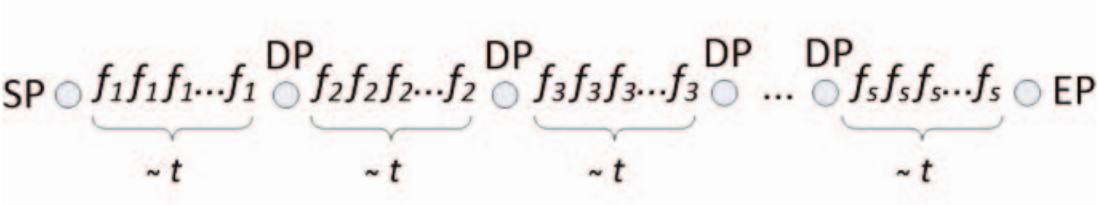
\includegraphics[width=\linewidth]{other/fuzzy.png}
\end{figure}

	\setsubsection{Conclusion}

		La méthode des points distincts est encore aujourd'hui exploré mais jusqu'à présent elle n'a pas donné de résultat probant. Une autre méthode pour limiter le coût des recherches dans les tables a été présenté par \cite{checkpoints} en 2005. C'est une méthode basé sur des points de contrôle. Nous la verrons plus en détail dans la prochaine section
		
\endinput{}

		\setsection{Améliorations notables : fausses alertes et outils de mesure}
	Comme nous l'avons vue précédement (section 3) le problème de fusion de chaîne a amené a créé les \glspl{rainbow}. Mais il se peut aussi qu'il y ait collision entre la chaîne que nous générons et une des chaînes des tables. Lorsque ce cas arrive nous parlons de fausse alertes.
	De plus jusqu'à présent nous n'avons pas réellement présenté d'outils permettant de comparer les efficacités des différentes méthodes de compromis.

\setsubsection{Points de contrôles}
	Afin de vérifier que 2 chaînes ne fusionnent il a été proposé par \cite{checkpoints} d'instaurer des points de contrôles. Pour ce faire $\alpha_i$ positions sont fixées. Pour chaque chaîne, la fonction G est évaluée et la valeur est stockée, à chacune de ces positions. Lors de la génération de la chaîne $Y_1,Y_2,...,Y_s$ nous évaluons également les $G(Y_{\alpha_i+s-t})$. La moindre différence entre les points de contrôles de cette chaîne et celle de la table correspond à une fausse alerte.

\begin{figure}
	\begin{minipage}{.5\textwidth}
		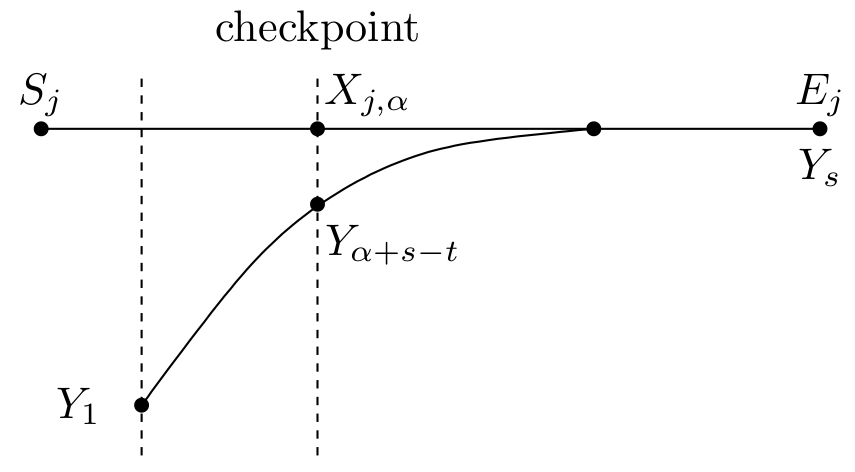
\includegraphics[width=0.9\linewidth]{other/FalseAlarmDetected.png}
		%\captionof{figure}{Fausse alerte détecté avec une probabilité de 1/2}
	\end{minipage}
	\begin{minipage}{.5\textwidth}
	    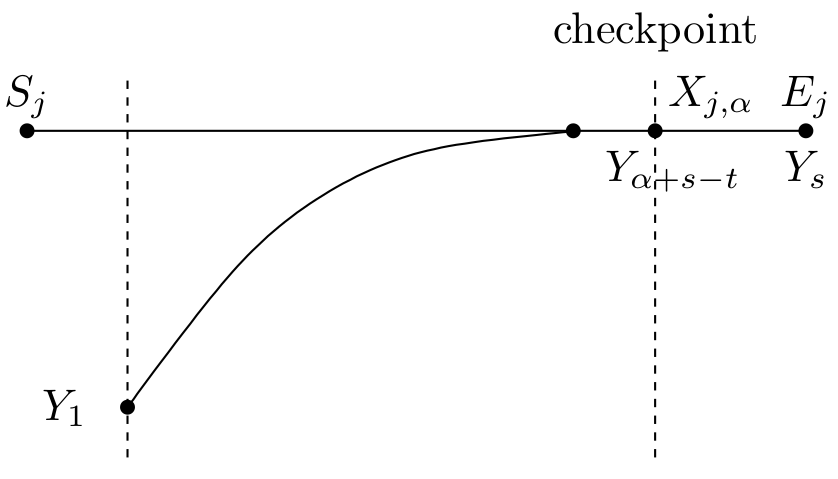
\includegraphics[width=0.9\linewidth]{other/FalseAlarmNotDetected.png}
		%\caption{Fausse alerte non détecté}
  	\end{minipage}
\end{figure}

	\bigskip
	
	les points de contrôle doivent être simple à évaluer et stocker, il est considéré que g sort les bits les moins significatifs. nous estimons selon la formule suivante la détection d'une fausse alerte :
\begin{align*}
pr\{g(x_{j,\alpha}) \neq g(y_{\alpha +s-t}) \mid x_{j,a} \neq y_{\alpha+s-t}\}=\frac{1}{2}(1-\frac{1}{2^{\mid k \mid}}) \approx \frac{1}{2}
\end{align*}




\setsubsection{Outils de comparaison}
	

\setsubsection{Conclusion}


\endinput{}

		\setsection{Conclusion}

	Nous avons vue l'introduction des \gls{TMTO} par Hellman en 1980, qui est une idée totalement novatrice. Puis, une nouvelle version de cette méthode proposé par Oeschlin en 2003 avec les \glspl{rainbow}. Entre temps la méthode des points distincts, proposé par Rivest en 1982, a été améliorée à différents reprise sans jamais être équivalente aux \glspl{rainbow}. Enfin nous avons découvert les points de contrôles et les tables parfaites, ainsi que l'équation permettant de comparer les différentes méthodes de compromis.

	\bigskip

	Il ressort de cette étude des différentes méthode de \gls{TMTO} que pour l'instant la méthode des \glspl{rainbow} est la méthode offrant généralement la meilleure solution. Même si la recherche reste active, cette méthode semble être la meilleure que nous puissions obtenir sans exploiter la forme de la fonction à inverser.

	\bigskip

	Jusqu'à présent ces méthodes étaient surtout connues pour permettre d'inverser une fonction de hachage, et ainsi attaquer les bases de données où sont stockés les mots de passes hashés. Mais pour faire à ce type d'attaque, un suffixe est ajouté aux mots de passe avant la phase de hashage, il s'agit du sel. Il faut alors reconstitué notre \gls{rainbow} pour chaque sel différent. Ceci étant dit il peut être utile cela peut être intéressant car les bases de données attaqués contiennent généralement des milliers de mots de passes.
	\bigskip
	Une autre utilisation des \gls{TMTO} qui pour l'instant ne semble pas trop utilisé est l'attaque par mot en clair choisie pour inverser une clé de chiffrement tel que proposé par Hellman.
	\bigskip
	Au-delà, de leurs intérêts en attaque informatique, les \gls{TMTO} sont également d'excellent outils à étudier d'un point de vue mathématiques. Et c'est pour toutes ces raisons que nous pensons que ces méthodes ne vont pas disparaître d'ici peu. 

\endinput{}


	\bibliographystyle{plain}

\end{document}
